\section[Propiedades]{Propiedades de los números aleatorios}
\begin{frame}{Introducción}
    \begin{itemize}
        \item Para desarrollar un modelo de simulación el ingrediente fundamental es la generación de una secuencia de números aleatorios $R_1, R_2, \dots , R_n$ \cite{BCN}.
        %\item La mayoría de los lenguajes de computador tienen una subrutina, objecto o función capaz de generar números aleatorios \cite{BCN}.
    \end{itemize}
\end{frame}

\begin{frame}{Propiedades de los números aleatorios}
    \begin{itemize}
        %\item Una secuencia de números aleatorios $R_1, R_2, \dots$, debe tener dos propiedades estadísticas importantes: uniformidad e independencia \cite{BCN}.
        
        \item Cada número aleatorio $R_i$ debe ser una muestra \textit{independiente} obtenida de una distribución \textit{uniforme} continua entre cero y uno \cite{BCN}.
        
    \end{itemize}
\end{frame}

\begin{frame}{Propiedades de la distribución uniforme $\left[0,1\right]$}
    $\begin{array}{ccc}
        f(x)=\left\{\begin{array}{cl}
        1, & 0\leq x \leq 1  \\
        0, & \text{de lo contrario}
    \end{array}\right.; & E(R)=\frac{1}{2}; & V(R)=\frac{1}{12}
    \end{array}$
    %\vskip-4pt
    \begin{columns}
        \begin{column}{0.5\textwidth}
            \begin{figure}
                \centering
                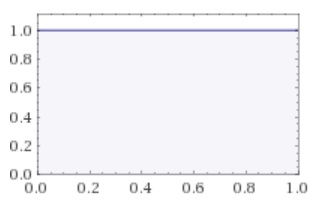
\includegraphics[width=5cm]{images/uniform_pdf.jpg}
                \caption{Función de densidad de probabilidad}
                \label{fig:pdf}
            \end{figure}
        \end{column}
        \begin{column}{0.5\textwidth}
            \begin{figure}
                \centering
                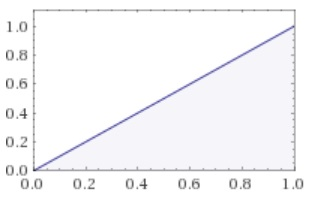
\includegraphics[width=5cm]{images/uniform_cdf.jpg}
                \caption{Función de probabilidad acumulada}
                \label{fig:cdf}
            \end{figure}
        \end{column}
    \end{columns}
\end{frame}
